% Generated by code/scripts/report_figures.py at 2026-11-10T17:41:22Z; do not edit.
% Inputs: artifacts/cluster/runs/bench4-20261110T103706Z-1535991
\begin{figure}[t]
\centering
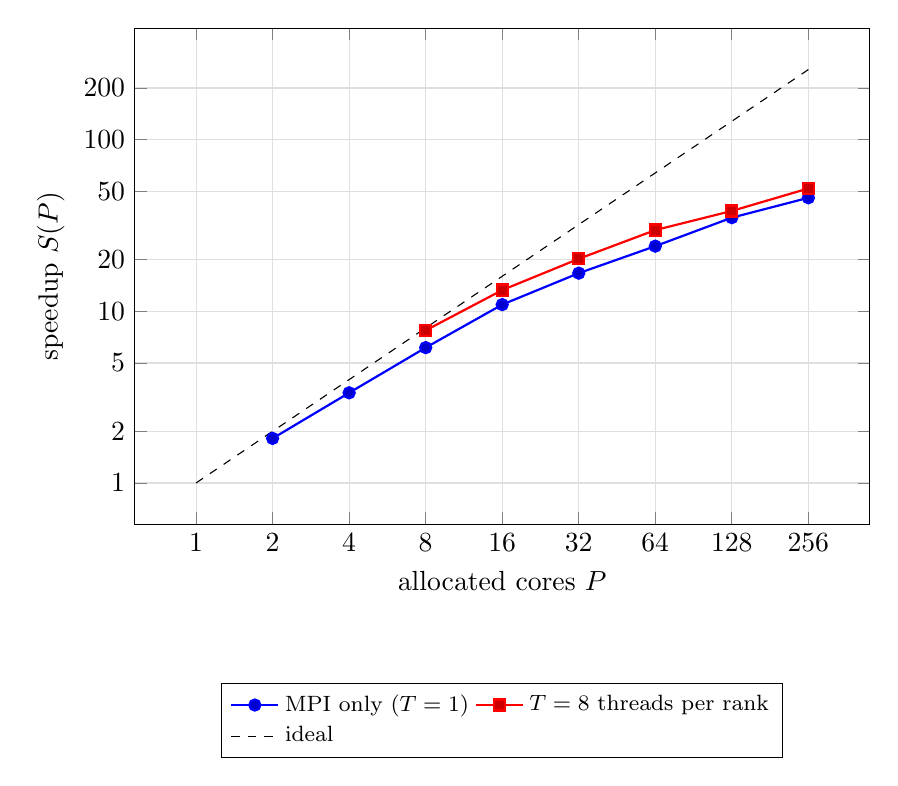
\begin{tikzpicture}
\begin{axis}[width=0.9\columnwidth, height=0.65\columnwidth, xlabel={allocated cores $P$}, ylabel={speedup $S(P)$}, xmode=log, log basis x=2, log ticks with fixed point, ymode=log, ytick={1,2,5,10,20,50,100,200,500}, legend style={at={(0.5,-0.32)}, anchor=north, legend columns=2, font=\footnotesize}, legend cell align=left, grid=major, grid style={gray!25}]
\addplot+[mark=*, thick] coordinates {(2,1.818) (4,3.351) (8,6.143) (16,10.94) (32,16.68) (64,23.96) (128,35.12) (256,45.84)};
\addlegendentry{MPI only ($T=1$)}
\addplot+[mark=square*, thick] coordinates {(8,7.741) (16,13.29) (32,20.22) (64,29.72) (128,38.43) (256,51.97)};
\addlegendentry{$T=8$ threads per rank}
\addplot[black, dashed] coordinates {(1,1) (256,256)};
\addlegendentry{ideal}
\end{axis}
\end{tikzpicture}
\caption{Strong-scaling speedup. $N=1000000$, median of repetitions; serial Barnes--Hut baseline on the same CPU model and build. Vanda job 1535991: 64 of 72 cores on each of four Platinum 8452Y nodes (CN-047, CN-061, CN-064, CN-065), 3 interleaved repetitions.}
\label{fig:b4-strong-speedup}
\end{figure}
